\newpage\subsection{Diseño del eje}
Para el diseño del eje se consideraron las cargas que los engranajes y rodamientos producen sobre este, tales fuerzas se obtuvieron teniendo en cuenta el engranaje con mayor potencia de transmisión y su velocidad de operación.

\begin{figure}[ht!]
    \centering
    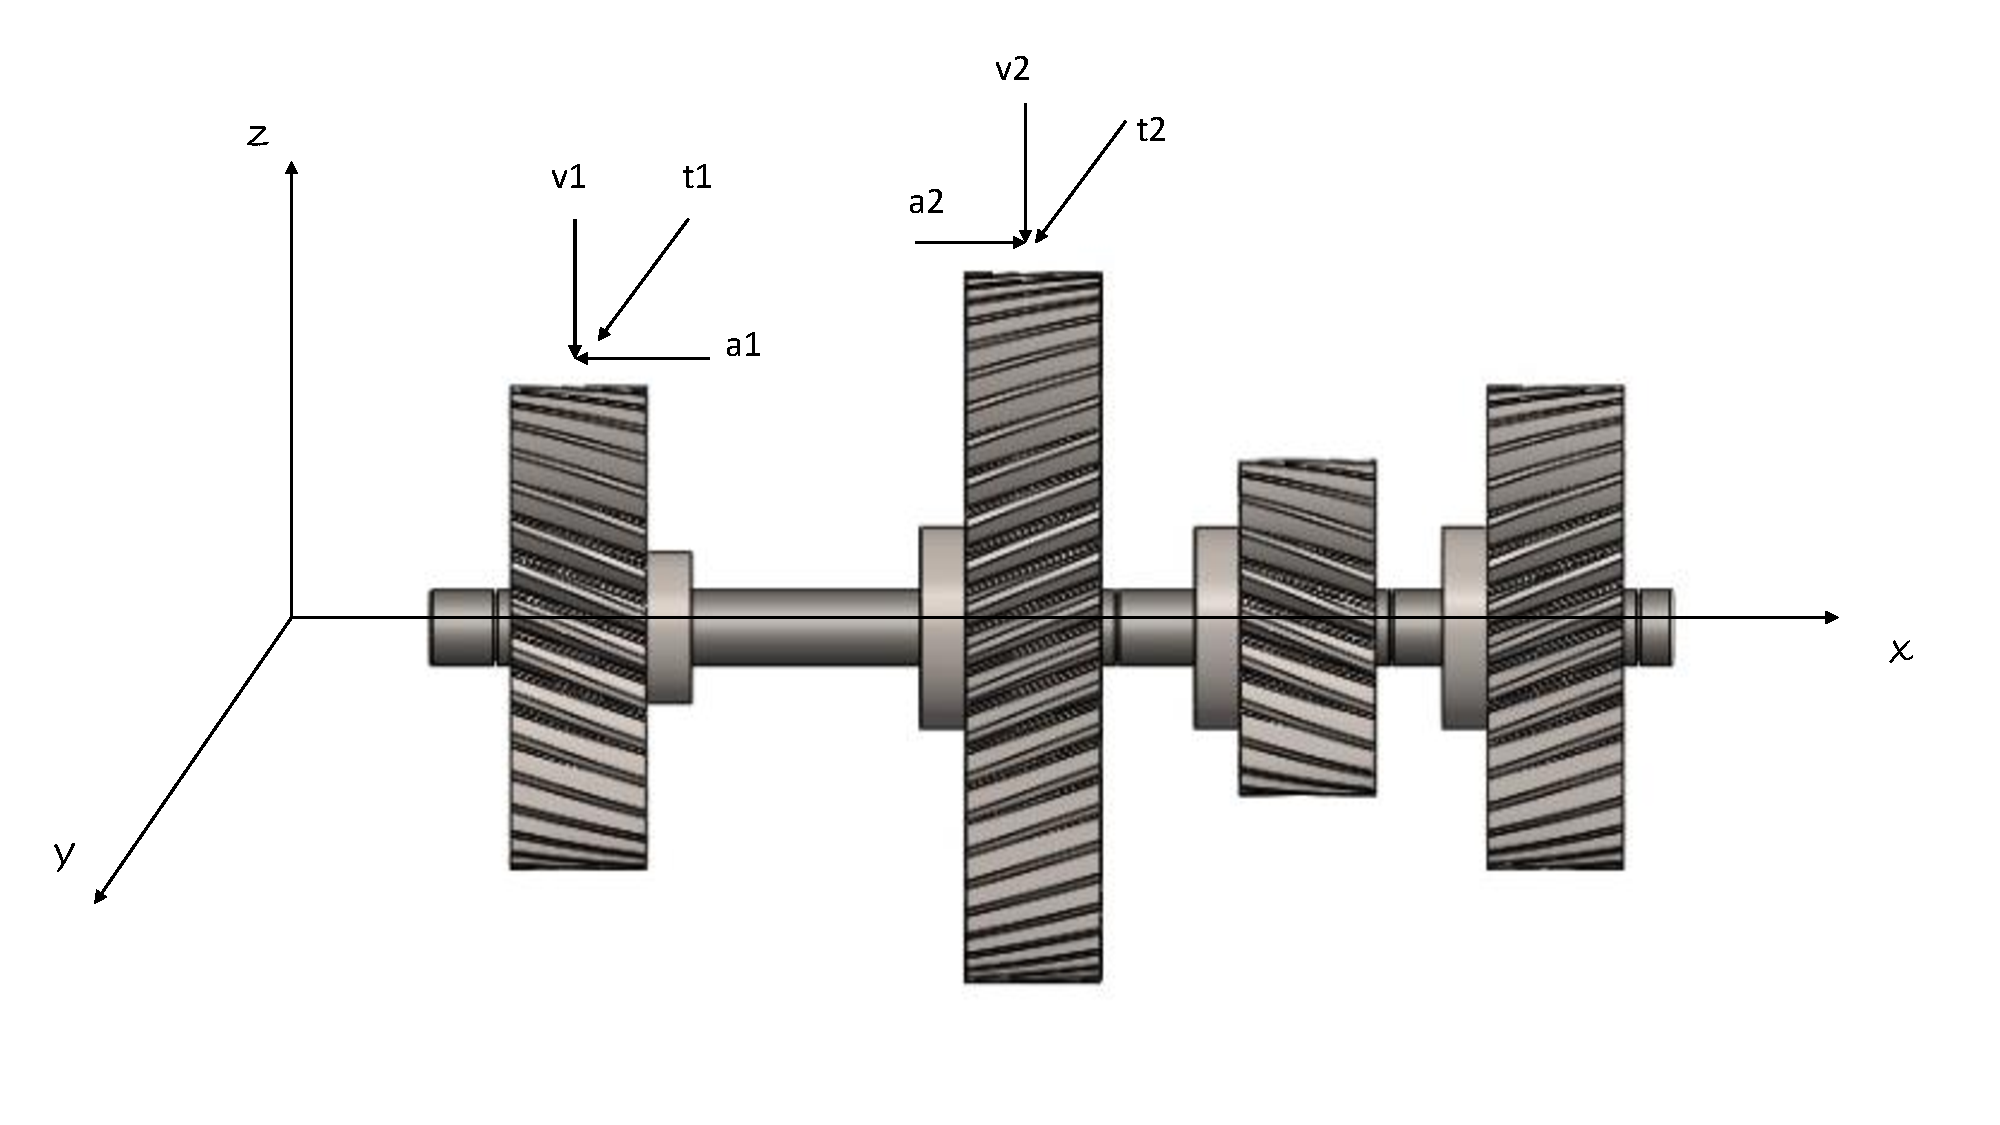
\includegraphics[height = 0.4\textheight,width=0.8\textwidth]{Cap5_DisenoDetallado/Figuras/Eje/DCL.pdf}
    \caption{DCL eje}
    \label{fig:DCL eje}
\end{figure}

%%%%% Tablas -------------------------------------------
\begin{longtable}{|c|c|c|c|c|c|c|c|c|c|c|c|}
\hline
Etapa & x mm  & r mm  & t N  & a N & v N & Fa Nmm  & Tt Nmm \begin{tabular}[c]{@{}c@{}}\end{tabular} \\ \hline
1          & 45      & 42.5 & 164.77  & 59.97 & 63.81 & 2548.7 & 7002.7 \\ \hline
2          & 146     & 63.75 & 109.85 & 39.98 & 42.54 & 2548.9 & 7002.9  \\ \hline

\caption{ Fuerzas y momentos sobre el Eje}{Fuente:Elaboracion Propia}
\label{table:fuerzas eje}
\end{longtable}
%% Plano xz -------------------------------------
\begin{figure}[ht!]
    \centering
    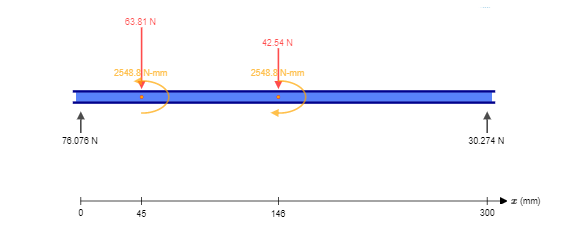
\includegraphics{Cap5_DisenoDetallado/Figuras/Eje/ejexz.PNG}
    \caption{DCL plano xz}
    \label{fig:ejexz}
\end{figure}

\begin{figure}[ht!]
    \centering
    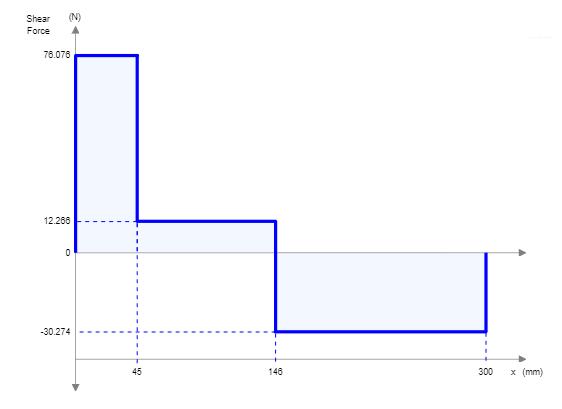
\includegraphics{Cap5_DisenoDetallado/Figuras/Eje/Vxz.PNG}
    \caption{Cortante en plano xz}
    \label{fig:Vxz}
\end{figure}
\newpage
~
\newpage
\begin{figure}[ht!]
    \centering
    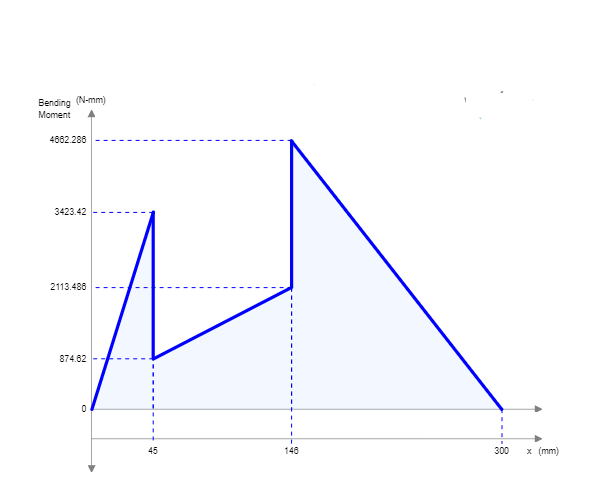
\includegraphics{Cap5_DisenoDetallado/Figuras/Eje/Flectorxz.PNG}
    \caption{Momento en plano xz}
    \label{fig:Fxz}
\end{figure}

%% Plano xy -------------------------------------

\begin{figure}[htb!]
    \centering
    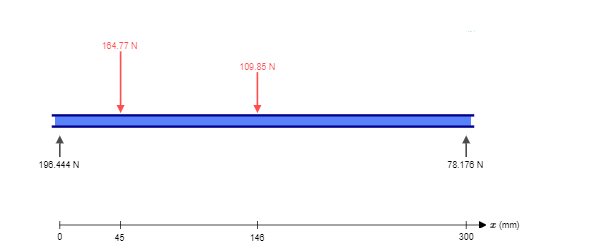
\includegraphics{Cap5_DisenoDetallado/Figuras/Eje/ejexy.PNG}
    \caption{DCL plano xy}
    \label{fig:ejexy}
\end{figure}

\begin{figure}[ht!]
    \centering
    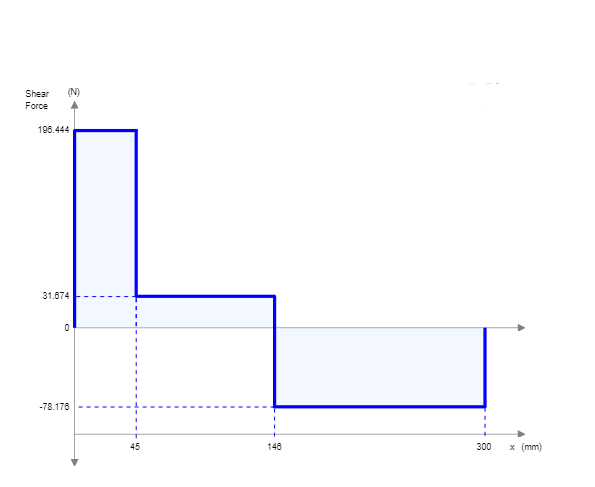
\includegraphics[height = 0.4\textheight,width=0.8\textwidth]{Cap5_DisenoDetallado/Figuras/Eje/Vxy.PNG}
    \caption{Cortante en plano xy}
    \label{fig:Vxy}
\end{figure}

\begin{figure}[ht!]
    \centering
    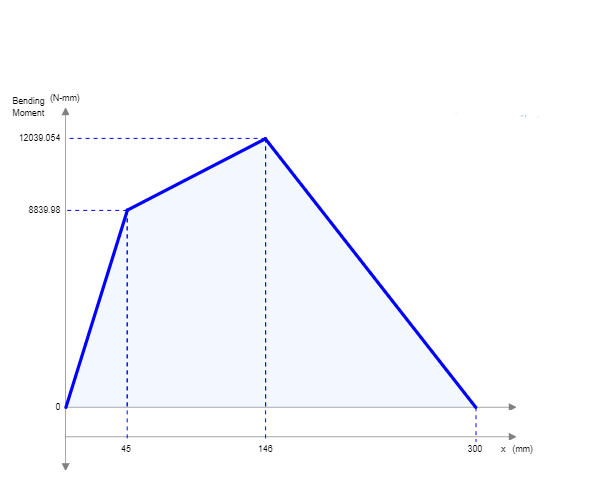
\includegraphics[height = 0.4\textheight,width=0.8\textwidth]{Cap5_DisenoDetallado/Figuras/Eje/Flectorxy.PNG}
    \caption{Momento en plano xy}
    \label{fig:Fxy}
\end{figure}
\newpage
~
\newpage
%%% ------------------------------
Se va a evaluar el punto donde el momento flexionante es máximo, es decir x = 146 mm, para lo cual se combinan los planos ortogonales como vectores y asi obtener un momento total $M_a = 12912 N.mm$ y torque medio $T_m = 7002 N.mm$
Teniendo en cuenta el momento alternante y torque medio obtenidos se puede evaluar la ecuación de Goodman Modificado reemplazando en ella los esfuerzos de Von Mises y despejando el diámetro del eje, resultando en la siguiente ecuación \citep{shigley2011shigley}:

\begin{equation}
    d = \left( \frac{16n}{\pi} \left\{ \frac{1}{S_e} [4(K_f M_a)^2 + 3(K_{fs} T_a)^2]^{1/2}   +       
                    \frac{1}{S_{ut}} [4(K_f M_m)^2 + 3(K_{fs} T_m)^2]^{1/2}     \right\} \right)^{1/3}
\end{equation}

Donde:\newline
$\textbf{S}_{ut}$ = 900 Mpa Acero AISI 4140\newline
Factor acabado superficial  $\textbf{K}_{a}$ = maquinado $4.51S_{ut}^{-0.265}$ = 0.7435 \newline
Factor de tamaño $\textbf{K}_{b}$ =  $1.24d^{-0.107}$ = 0.9281 \newline
Factor de carga $\textbf{K}_{c}$ = 1 \newline
Factor de temperatura $\textbf{K}_{d}$ = 1 \newline
Factor de Confiabilidad $\textbf{K}_{e}$ = 0.753    para una confiabilidad de 99.9\%\newline
Factor de efectos varios $\textbf{K}_{c}$ = 1 \newline
Limite de resistencia a la fatiga en viga rotatoria $\textbf{S'}_{e}$ = $0.5S_{ut}$ para $S_{ut} < 1400 Mpa$ \newline
Límite de resistencia a la fatiga en la ubicación crítica $\textbf{S}_{e}$ =\newline
Factor de Seguridad n = 2 \newline

Teniendo en cuenta los valores de sensibilidad de la muesca $q = 0.8$ , $ q_c = 0.85$ y factores de concentración de esfuerzo $K_t = 1.6$, $K_{ts} = 1.4$ tomados de Shigley 2011 se obtuvieron los valores de $K_f = 1.48 $ y $K_{fs}  = 1.38$ con la siguiente ecuación:

\begin{equation}
    K_f = 1 + q(K_t -1) 
\end{equation}

\begin{equation}
     K_{fs} = 1 + q_{c}(K_{ts} -1)
\end{equation}

Evaluando en la ecuación de diseño se encontró un diametro minimo de 12.5 mm, el cual se llevó a 15 mm por razones constructivas y con el cual se tiene un factor de seguridad de 3.5
